\documentclass[a4paper, 12pt]{scrartcl}
\usepackage[utf8]{inputenc}
\usepackage[ngerman]{babel}
\usepackage[T1]{fontenc}
\usepackage{graphicx}
\usepackage{hyperref}

\hypersetup{
	colorlinks=true,
	linkcolor=blue,
	filecolor=blue,      
	urlcolor=blue,
	pdftitle={ Example},
	pdfpagemode=FullScreen,
}

\title{End-2-End-Prozess}
\titlehead{Praxisbericht}
\author{Maksym Mykhailych}
\date{09. September 2025}

\begin{document}
	\maketitle
	\newpage 	
	\tableofcontents
	\newpage
	%\section{Abstract}
	
	\newpage
	\section{Einleitung}
	Einleitender Text.
	\newpage
	\subsection{Motivation}
	\subsection{Aufgabenstellung}
	\subsection{Aufbau der Arbeit}
	Text.
	\newpage
	\section{Grundlagen}
	\subsection{Vorstellung von Capgemini}
	\subsubsection{Gesamtheitliche Darstellung von Capgemini} %VOrstellung von Capgemini(Geschichte, Zahlen, Wie groß?)
Capgemini, mit Hauptsitz in Paris, ist ein transnationales, börsennotiertes Unternehmen, das Beratungs-, Technologiedienstleistungen und digitale Transformationslösungen anbietet. Das Unternehmen bietet eine Vielzahl von Dienstleistungen, darunter Beratung, Technologie und Outsourcing. Mit einer Präsenz in über 50 Ländern bedient Capgemini Kunden aus diversen Branchen, einschließlich Finanzdienstleistungen, Automobilindustrie, Gesundheitswesen und Einzelhandel. Im Jahr 2023 erzielte Capgemini einen Umsatz von 22,5 Milliarden Euro und beschäftigt weltweit etwa 340.000 Mitarbeiter, davon rund 12.500 in Deutschland laut der internen Daten.
	\begin{figure}[h!]
		\begin{center}
			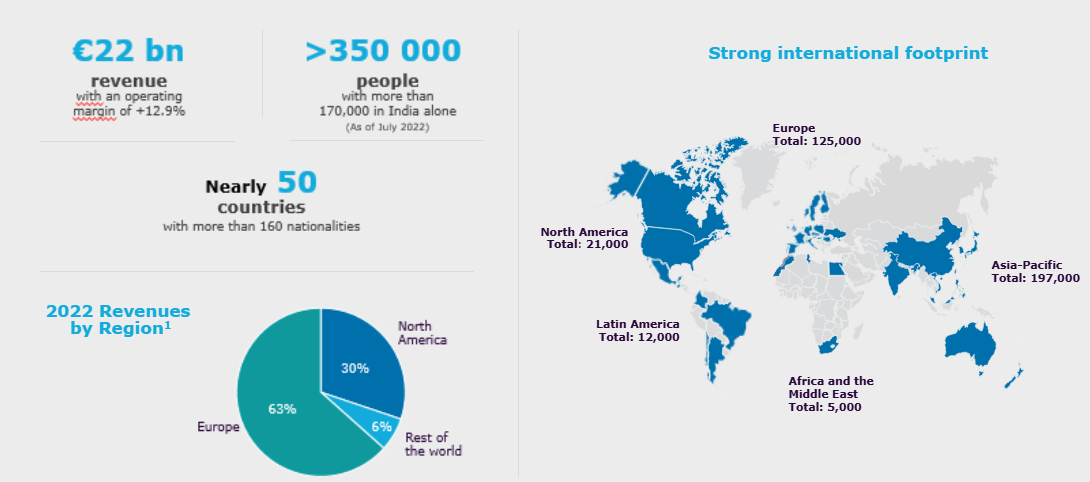
\includegraphics[width=12cm]{CApgemini zahlen.png}
			\caption{Stand von Capgemini zu 2023}
			\label{Stand von Capgemini}
		\end{center}
	\end{figure}
	\subsubsection{Struktur und Organisation in Deutschland}

Capgemini bietet ihren Kunden eine End-to-End-IT-Transformation, die von der Umgestaltung komplexer IT-Architekturen bis hin zur Entwicklung spezifischer kleiner Funktionen reicht. In diesem Zusammenhang verfügt Capgemini über eine komplexe Matrixstruktur. Abbildung~\ref{fig:Matrix Struktur} zeigt, dass BU Deutschland sich in drei große Geschäftseinheiten GBL(Globale Business Lines), ABL(Application Business Lines) und MU(Market Unit) unterteilt.
	\newpage
	\begin{figure}[h]
		\begin{center}
			\includegraphics[width=10cm]{BU Germany CAP.png}
			\caption{Matrix Struktur von Capgemini}
			\label{fig:Matrix Struktur}
		\end{center}
	\begin{itemize}
		\item MU ist für die Gewinnung des Projektes zuständing. Sie sind eine Schnittstelle zwischen den Kunden und Capgemini sog. "Demand" Manager. 
	\end{itemize}
	\end{figure}
	\newpage
	\subsection{Definition des End-2-End-Prozesses}
	\subsubsection{Überblick des allgemeinen End-2-End-Prozesses} %wie sieht algemein E2E-Prozess bei der Beratung!

	\subsubsection{End-2-End-Prozess bei Capgemini}
	\subsection{PLM-Systeme}
	\subsubsection{Allgemeine Übersicht der PLM-Systeme}
	\subsubsection{Vorstellung von verschiedenen Vendoren}
	Text.
	\newpage
	\section{Durchführung}
	\subsection{Phase 1: Sales} 
	\subsubsection{Ausgangslage und Aufgabenstallung} %Ich beschäftige mich mit der Showcase für die Kunden um das Projekt zu kriegen.
	\subsubsection{Anforderungen für die Erstellung der Demonstratorenübersicht} %welche versionen die Demonstratoren haben, Ziel des Demonstrators, Beschreibungen etc.
	\subsubsection{Tools-Analyse}%Welche Tools gibt und welche sind geeignet für meinen Demostrator(Beschränung von Unternehmen betrachten)
	\subsubsection{Erstellung der Demonstratorenübersicht}
	\newpage
	\subsection{Phase 2: Staffing}
	\subsubsection{Relevanz der Staffing für Capgemini}%was lebenswichtiges macht Christoph
	\subsubsection{Ausgangslage und Aufgabenstellung}
	\subsubsection{Anforderungen fürs Reporting}
	\subsubsection{Umsetzung des Berichtswesen...}
	\newpage
	\subsection{Phase 3: Projektplanung}
	\newpage
	\subsection{Phase 4: Delivery}
	\newpage
	\subsection{Phase 5: Closure}
	\newpage
	\section{Auswertung}
	\subsection{Validierung der Anforderung}%für PLM
	\newpage
	\section{Ergebnisse und Diskussion}
		\newpage
	\section{Ausblick}
	asdasdasdasda~\cite{karmasin2017gestaltung}
	asdasdasdasda~\cite{example2025}
		\newpage
	\section{Anhang}
	\bibliographystyle{plain}
	\bibliography{Gestaltung_wissenschaftlicher_Arbeit.bib}
	\subsection{Anforderungen für das Showcase}
	\begin{itemize}
		\item Zielsetung und Planung
		\item Infrstraktur aufbauen
		\subitem PDM-systeme und PLM-software auswählen
		\subitem CAD-Tools integrieren
		\subitem ERP-Systeme 
		\item Erstellung der Demonstrationsdaten
		\subitem Beispielprodukt entwickeln nach Zielsetzung
		\subitem Stückliste für das Produkt vorbereiten
		\item Visualisierung entwickeln
		\item Tests durchführen
		\item Präsentation für die Entwicklung des Beispielprodukts vorbereiten 
	\end{itemize}
\end{document}